%to have line numbers
%\RequirePackage{lineno}
\documentclass[10pt, letterpaper]{article}      
\usepackage[margin=.1cm,font=small,labelfont=bf]{caption}[2007/03/09]
%\usepackage{endnotes}
\usepackage{setspace}
\usepackage{longtable}                        
\usepackage{anysize}                          
\usepackage{natbib}                           
%\bibpunct{(}{)}{,}{a}{,}{,}                   
\bibpunct{(}{)}{,}{a}{}{,}                   
\usepackage{amsmath}
\usepackage[pdftex]{graphicx}                
\usepackage{epstopdf}
\usepackage{hyperref}                             % For creating hyperlinks in cross references


% \usepackage[margins]{trackchanges}

% \note[editor]{The note}
% \annote[editor]{Text to annotate}{The note}
%    \add[editor]{Text to add}
% \remove[editor]{Text to remove}
% \change[editor]{Text to remove}{Text to add}



\marginsize{1cm}{1cm}{.5cm}{.5cm}%{left}{right}{top}{bottom}   
					          % Helps LaTeX put figures where YOU want
 \renewcommand{\topfraction}{1}	                  % 90% of page top can be a float
 \renewcommand{\bottomfraction}{1}	          % 90% of page bottom can be a float
 \renewcommand{\textfraction}{0.0}	          % only 10% of page must to be text

 \usepackage{float}                               %latex will not complain to include float after float

\usepackage[table]{xcolor}                        %for table shading
\definecolor{gray90}{gray}{0.90}
\definecolor{orange}{RGB}{255,128,0}

\renewcommand\arraystretch{.9}                    %for spacing of arrays like tabular

%-------------------- my commands -----------------------------------------
\newenvironment{ig}[1]{
\begin{center}
 %\includegraphics[height=5.0in]{#1} 
 \includegraphics[height=3.3in]{#1}
\end{center}}

 \newcommand{\cc}[1]{
\hspace{-.13in}$\bullet$\marginpar{\begin{spacing}{.6}\begin{footnotesize}{#1}\end{footnotesize}\end{spacing}}
\hspace{-.13in} }

%-------------------- END my commands -----------------------------------------



%-------------------- extra options -----------------------------------------

%%%%%%%%%%%%%
% footnotes %
%%%%%%%%%%%%%

%\long\def\symbolfootnote[#1]#2{\begingroup% %these can be used to make footnote  nonnumeric asterick, dagger etc
%\def\thefootnote{\fnsymbol{footnote}}\footnote[#1]{#2}\endgroup}	%see: http://help-csli.stanford.edu/tex/latex-footnotes.shtml

%%%%%%%%%%%
% spacing %
%%%%%%%%%%%

% \abovecaptionskip: space above caption
% \belowcaptionskip: space below caption
%\oddsidemargin 0cm
%\evensidemargin 0cm

%%%%%%%%%
% style %
%%%%%%%%%

%\pagestyle{myheadings}         % Option to put page headers
                               % Needed \documentclass[a4paper,twoside]{article}
%\markboth{{\small\it Politics and Life Satisfaction }}
%{{\small\it Adam Okulicz-Kozaryn} }

%\headsep 1.5cm
% \pagestyle{empty}			% no page numbers
% \parindent  15.mm			% indent paragraph by this much
% \parskip     2.mm			% space between paragraphs
% \mathindent 20.mm			% indent math equations by this much

%%%%%%%%%%%%%%%%%%
% extra packages %
%%%%%%%%%%%%%%%%%%

\usepackage{datetime}


\usepackage[latin1]{inputenc}
\usepackage{tikz}
\usetikzlibrary{shapes,arrows,backgrounds}


%\usepackage{color}					% For creating coloured text and background
%\usepackage{float}
\usepackage{subfig}                                     % for combined figures

\renewcommand{\ss}[1]{{\colorbox{blue}{\bf \color{white}{#1}}}}
\newcommand{\ee}[1]{\endnote{\vspace{-.10in}\begin{spacing}{1.0}{\normalsize #1}\end{spacing}\vspace{.20in}}}




\usepackage{sectsty}
\allsectionsfont{\normalfont\sffamily}



\usepackage{sectsty}
\allsectionsfont{\normalfont\sffamily}
\usepackage[margins]{trackchanges}

\renewcommand\familydefault{\sfdefault}

\usepackage{verbatim}
\usepackage{rotating}
\usepackage{catchfilebetweentags}
%-------------------- END extra options -----------------------------------------
\date{Draft: {}\today}
\title{
%  The Paradox of Energy Consumption and Happiness Across Countries
Energy Use And Happiness
}
\author{
Adam Okulicz-Kozaryn\thanks{EMAIL: adam.okulicz.kozaryn@gmail.com
  \hfill I thank XXX.  All mistakes are mine.} \\
{\small Rutgers - Camden}\\
Micah Altman\thanks{EMAIL: ???
  \hfill I ???} \\
{\small MIT}
}

\begin{document}

%%\setpagewiselinenumbers
%\modulolinenumbers[1]
%\linenumbers

%\bibliographystyle{/home/aok/papers/root/tex/ecta}
\maketitle
\vspace{-.4in}
\begin{center}

\end{center}

\begin{abstract}
\noindent Perhaps the biggest gap in large happiness literature is
consumption--we know little about the effect of consumtion on happiness. Energy
consumption is critical for many reasons.  We study energy use and happiness across countries.  Energy
use is defined as total enery used in a country per capita. Happiness data come
 from World Values Survey. There are striking severalfold differences in
energy use. The bivariate relationship conforms to a traditional tradeoff--the
more energy we consume, the happier we are, and hence energy conservation faces
a tradeoff in wellbeing. This apparent relationship disappears, however, when
income is taken into account. Furthermore, we find that the relationship becomes
positive again when $CO_2$ emissions are taken into account. We interpret this
 as another argument to curb pollution and conserve natural resources, but also
 as an argument in favor of renevable or clean energy sources, say wind or solar.  %MAYBE or LATER can  control for clean energy
 Fundamentally, the ultimate goal of increased energy consumption is human
 happiness--if there is no increased happiness because energy consumption
 pollutes, then we should either consume less or consume cleaner. We discuss directions for future research.
\end{abstract}
\vspace{.15in} 
\noindent{\sc keywords:  energy use,  sustainability, wellbeing,
  happiness, Subjective Well-Being (SWB)}
%\vspace{-.25in} 

\begin{spacing}{1.4}
\rowcolors{1}{white}{gray90}

%  \ExecuteMetaData[../out/tex]{ginipov}

% \begin{figure}[H]
%  \includegraphics[height=3in]{../out/gov_res_trust.pdf}\centering\label{gov_res_trust}
% \caption{woo}
% \end{figure}

\section{Introduction}

A very fundamental question is how to achieve both happiness and
sustainability--it is difficult because there appears to be a tradeoff.
Fundamentally,
 the ultimate goal of increased energy consumption is human
 happiness--if there is no relationship between the two, then we can
 consume less and stay happy.

Energy consumption is important--countries wage wars about energy sources. Many
countries' whole economies are based on energy exports (e.g. OPEC
countries). Many other countries rely heavily on energy production and some use
it as a political tool, e.g. Russia. 
Virtually all countries  always seek to get more--a recent example is so called
fracking. Yet, we need more focus of on conservation. There are at least two
obvious reasons--most of energy consumed today is non-renewable--it comes from
fossil fuels and they will run out sooner or later. %TODO be specific give numbers
Second, energy consumption results in pollution and pollution is bad not only
for environment and other species but also for us, the beneficiaries of energy
consumption, and thus it potentially cancels out the benefits of energy
consumption. The basic idea is that if there is not much happiness gained from
energy consumption then it would be another reason for energy
conservation. 
In this descriptive correlational study we aim to paint the picture and
encourage more research in the area this underexplored area.

A recent report by
Intergovernmental Panel on Climate Change is alarming 
(\url{http://www.ipcc.ch/}). Indeed, a threat is serious enough that
claims for not growing the economy anymore or even ``degrowing'' it
appear reasonable \citep{kallis12}.\footnote{Although it is not
  immediately obvious what is the best strategy to achieve greater
  sustainability--degrowth \citep{kallis11} or simply public policy
  \citep{bergh11}--for more discussion see \citet{daly13,kallis12}.} At very
least curbing consumption is a reasonable soution, perhaps even as high as by
factor of 10 in affluent societies  as advocated by \citet{pretty13}. This,
of course, begs a question, what would happen to our happiness?


\section{The Happiness-Energy Conservation Tradeoff?}

A common or received wisdom is that there is a tradeoff between happiness and
energy use--we need to consume energy in order to achieve greater
happiness. One could even say, that the very end goal (usually implicit though)
of energy consumption is happiness. \footnote{On the other hand, energy results in pollution, which
  decreases happiness \citep[e.g]{welsch05, weinhold12}.} This is
true in buivaraite case--the richer areas are happier.
 We argue here that it is not necassarily so, only after taking into account
 income at country level % and few other variables at state or county levels,
 the relationship between energy consymptiona nd happiness disappears.

% its striking 2 fold or more differences between states like nj and tx and only a
% small fracton of that is due to climate most due to consumption arguably
% wateful/conspicous--calculate how mich explained by climate! give number

Arguably a major if not key factor prohibiting us from conservation and
sustaiinability is fear of loss in wellbeing--we argue here that such loss will
not be great. Indeed, our results suggest that curbing energy use that results
in pollution, that is most of today's energy use, will not affect adversly our
happiness, because the unhappiness created by energy consumption cut will be
offset by happiness created by cut in pollution.  

There is anectodal evidence pointing to the fact that humans can live happily
without much energy--among Amish, African Maasai, and Greenlandic Inughuit, most
people are above neutral in well-being.

But what is the mechanism? Why energy consumption is not likely to buy much
hppiness? We already mentioned one: pollution--energy cnsumption and $CO_2$
emissions correlate at above .9, and pollution reduces happiness. But there are
also psychological causal pathways.
We should buy experience, not things--that's why probably energy
consumption in transportation brings most happiness because much of
transportation is experience --e.g. travel vacations etc. 
% TODO from ls\_car lsPol and: 
% Here psychological literature helps.
Simply material consumption (where
arguably most of the  the energy consumption falls) does not result in lasting
happiness as opposed to experiece consumption. Indeed, sustainable consumption
does not necessarily mean less happiness, and there are many examples of
activities low in carbon footprint but high in happiness such as gardening or
yoga \citep{madjar06}. 


\section{What Do We Know So Far? The Literature}

It is striking then that large happiness literature has omitted topic of energy
so far--threre are no studies about energy consumption and happiness across
areas, and only one study across persons.  \citet{graef81} (recently republished
as \citet{csikszentmihalyi14}) is the  only study about energy consumption and
happiness. This was a person-level study that used experience
sampling method (ESM) and it found no relationship between energy consumption
and happiness or even a negative relationship for females. 

Going back to initial question of how to achieve both happiness and
sustainabilty--we are not the first to try to answer it, we are only to fist to
do it using happiness and energy measures. Others used other measures.
Literature does look at the effect of energy consumption on human
wellbeing, but operationalizes human wellbeing differently--mostly as HDI or its
components. And literature proposes various indices linking HDI or its
components to natural resources or environment.

For instance, \citet{dietz09} proposed environmentally efficient wellbeing
(EWEB) as function of economic, natural and human resources. A simlar, but
closer to energy focus of present study is \citet{jorgenson14B} who proposed
energy intensity of human wellbeing. Yet, again, all of these approaches remain
in the realm of HDI or its components, GDP, education and life expectancy. 
 Using human development index (HDI) \citep{steinberger10} and argues along the
 same lines as present paper: increasing energy consumption beyond a point does
 not contribute anymore to wellbeing.  Many more studies link enrgy use to HDI
 \citep[e.g.]{dias06}, yet HDI, like  GDP, has its limitations--for an overview
 see \citet{klugman11}--and hence  recently happiness was proposed as another
 measure of broadly understood human  development--incidentally Amartya Sen both
 co-introduced HDI in 1990 and  reently advocatdes happiness \citep{stiglitz09al}. 

We will use happiness measure. But it is worth noting that there is also
 happy years measure (happiness$*$life expectancy) \citep{veenhoven96B}, and
 finally Happy Planet Index ($\frac{happiness*life\;expectancy}{ecological\;footprint}$)--this is somewaht close approach to  ours, except that we will try to see how energy consuption specifically afects  happiness. And there are few more: Genuine Progress Indicator, Ecological Footprints,  and planetary boundaries--see p. 477 in \citet{pretty13} for  sources. 

While there is no literature about energy use and happiness, there is related
literature. \citet{pretty13} provides a wonderful overview of the relationship
betweenresource consumption, economy and wellbing including happiness measure of
it. There is literature about relationship between happiness and outcomes
related to energy consumption or attitudes about consumption. First, pollution makes us unhappy \citep{weinhold12,welsch05}. Second,
and more important,  there is some evidence that happy people
are more sustainable, that is, happiness affects sustainability
\citep{ericson14}.  Causation possibly goes in the
other direction as well (as noted by authors), but in general it is
safe to say that happiness and sustainable behavior are correlated  \citep{brown05,corral11}.

Then there is energy efficiency that moderaters (or mediates?) the relationship
between energy use and happiness--it is not only that energy use that results in
happiness, but importantly its efficient use--one country may waste lots of
energy say due to outdated and inefficent technologies as those in 1990s in
Eastern Europe, whereas some other ountry can actually use less energy per
capita but actually deliver more wellebing because enrgey is better used. We
will accounty for  energy efficiency by controlling for  $CO_2$ emissions. 
 A country that can produce more energy with less $CO_2$ is more energy
 efficient--perhaps a crude measure but readily available for a large sample of
 countries. There are better measures (e.g. \url{http://www.aceee.org/research-report/e1402}) but available for only a handful of countries
%can
                                %also do co2 per gdp  guess also can do co2 per
                                %energy etc etc

A related issue is that of ``rebound problem'' or the Jevons paradox
\citep{pretty13}%p476-477
--efficiency frees up resources that are then used to increase consumption, and
hence technological progress or efficient technology by itself does not lead to
sustainability. While in the developed World, energy consumption is flat or even
decreasing, it is globally increasing due to the developing World
\citep{pretty13}. Energy consumption, like economic growth and consmption has no
limit--indeed, instead of satysfying our needs it stimulates them--''the more
one has the more one wants, since satisfactions received only stimulate instead
of filling needs''   \citep{durkheim50}. This brings us to three major happiness
theories, all relevant to this study. 

\section{The three happiness theories}

Before answering a question of how is happiness created, let's define it first. 
  Happiness, or the more scientific term Subjective Well-Being (SWB), is ``both cognitive judgments of one's life
satisfaction in addition to affective evaluations of mood and
emotions'' \citep[p. 142]{steel08},  or in other words: ``overall judgment of life that draws on two sources of information:
  cognitive comparison with standards of the good life (contentment) and
  affective information from how one feels most of the time (hedonic
  level of affect).''(\citep[p. 2]{veenhoven08})
 Some scholars make a
  distinction between happiness and life satisfaction--life
  satisfaction refers to cognition and happiness refers to affect. In practice,
  however, it is usually difficult  if not impossible to separate the two
  concepts.  Hence, the overall happiness definition by 
   \citet{veenhoven08}, as quoted above,  seems most appropriate and we will use terms
   ``happiness,''``life satisfaction'' and ``(subjective) wellbeing'' interchangeably.  For a recent and very through statement of
happiness measure validity and reliability see \citet{diener09}
(especially ch. 5). 

The adaptation theory \citep{brickman78cj} argues that there is
adjustment to external circumstances and we are on a 'hedonic
treadmill.' ``The more one has the more one wants, since satisfactions
received only stimulate instead of filling needs''\citep{durkheim50}. 
We arguably get used to (adapt to) energy consumption, too. Hence, increasing
energy consumption is futile for our happiness, because we will adapt to it and
always want more.
%
The  multiple discrepancy theory  \citep{michalos85} states that
happiness is a result of social comparison or a comparison to various
standards.  I compare my consumption to others. I also compare
it to standards--for instance, that of people in my geographic or social
proximity. Notably, this may result in consumption arms race--people wanting to
outcompete others in terms of consumption in a vicious
cycle \citep{frank12}. Hence, also like  per adaptation theory, energy consumtion
will not result in geater happiness.  
%
  The needs/livability theory \citep{veenhoven95, veenhoven14b} posits that
  happiness results from objective living conditions and from
  fulfillment of our needs, and predicts that higher physical or economic
  development will result in greater happiness. It is not clear, however, if
  there is any limit to the level of development that should result in greater
  happiness as it is not clear what is the limit to human needs. Of course, one
  could argue that there are needs and wants, and while there are some clearly
  defined needs (e.g. biological), most other needs are relative and
  subjective. Hence, based on this theory, as opposed to the other two theories,
  greater energy use will result in greater happiness.
  

\section{Data and Results}

We analyse data in a cross-ection--there is not much variation over time for
instance in US and West-European countries, %look at world.do: manheim or
                                %states.do for us states
 but there is lots of varaition across areas.

We use happiness data from World Values Survey
(\url{http://www.worldvaluessurvey.org/wvs.jsp})--we use a cumulative file
covering first 4 waves (1981-2007), hence some countries are observed more than
once. Happiness is averaged for each country-year and matched with energy use
and other  socioeconomic controls from World Bank
(\url{http://data.worldbank.org/indicator}). Table \ref{var_des} lists variables
used and their definitions.


\begin{table}[H]\centering\footnotesize
 \caption{\label{var_des} Variable definitions}
\begin{tabular} {p{1.5in}p{4.5in}}   \hline
name & description   \\ \hline
  happiness & "All things considered, how satisfied are you with your life as a whole these days?" 1="dissatisfied" to 10="satisfied"; WVS \\
  PCGDP & GDP per capita (constant 2005 US\$); Code: NY.GDP.PCAP.KD; "GDP per capita is gross domestic product divided by midyear population. GDP is the sum of gross value added by all resident producers in the economy plus any product taxes and minus any subsidies not included in the value of the products. It is calculated without making deductions for depreciation of fabricated assets or for depletion and degradation of natural resources. Data are in constant 2005 U.S. dollars."; WB \\
  energy use, pc & Energy use (kg of oil equivalent per capita); Code: EG.USE.PCAP.KG.OE "Energy use refers to use of primary energy before transformation to other end-use fuels, which is equal to indigenous production plus imports and stock changes, minus exports and fuels supplied to ships and aircraft engaged in international transport."; WB \\
  unemployment, \% & Unemployment, total (\% of total labor force) (modeled ILO estimate); Code: SL.UEM.TOTL.ZS; "Unemployment refers to the share of the labor force that is without work but available for and seeking employment."; WB \\
  co2 emissions, pc & CO2 emissions (metric tons per capita); Code: EN.ATM.CO2E.PC; "Carbon dioxide emissions are those stemming from the burning of fossil fuels and the manufacture of cement. They include carbon dioxide produced during consumption of solid, liquid, and gas fuels and gas flaring."; WB \\
  female life expectancy & Life expectancy at birth, female (years); Code: SP.DYN.LE00.FE.IN; "Life expectancy at birth indicates the number of years a newborn infant would live if prevailing patterns of mortality at the time of its birth were to stay the same throughout its life." WB\\
  road sector gasoline fuel consumption, pc & Road sector gasoline fuel consumption per capita (kg of oil equivalent); Code: IS.ROD.SGAS.PC; "Gasoline is light hydrocarbon oil use in internal combustion engine such as motor vehicles, excluding aircraft."; WB \\
  percent urban & population (\% of total); Code: SP.URB.TOTL.IN.ZS; "Urban population refers to people living in urban areas as defined by national statistical offices. It is calculated using World Bank population estimates and urban ratios from the United Nations World Urbanization Prospects." WB\\
  maximum temperature in January & "near-surface temperature maximum (degrees Celsius)" ; TYN\_CY \\
  maximum temperature in July & "near-surface temperature maximum (degrees Celsius)" ; TYN\_CY \\
\hline\end{tabular}\end{table}

{\scriptsize \noindent Variable sources. WVS: World Values Survey \url{www.worldvaluessurvey.org};
TYN\_CY: Tyndall Centre (\url{www.tyndall.ac.uk}) Mitchell,T.D., Hulme,M., and
New,M., 2002: Climate data for political areas. Area
34:109-112. \url{http://www.cru.uea.ac.uk/~timm/cty/obs/TYN_CY_1_1_var-table.html};
WB: World Bank \url{http://data.worldbank.org}}

% US STATES:
% There are large differences in energy use per capita accross states--twofold or
% larger, yet energy-hungry states are no happier (with possible exceptioon of
% transportation sector)--this is just another argument for energy conservation.

\begin{figure}[H]
 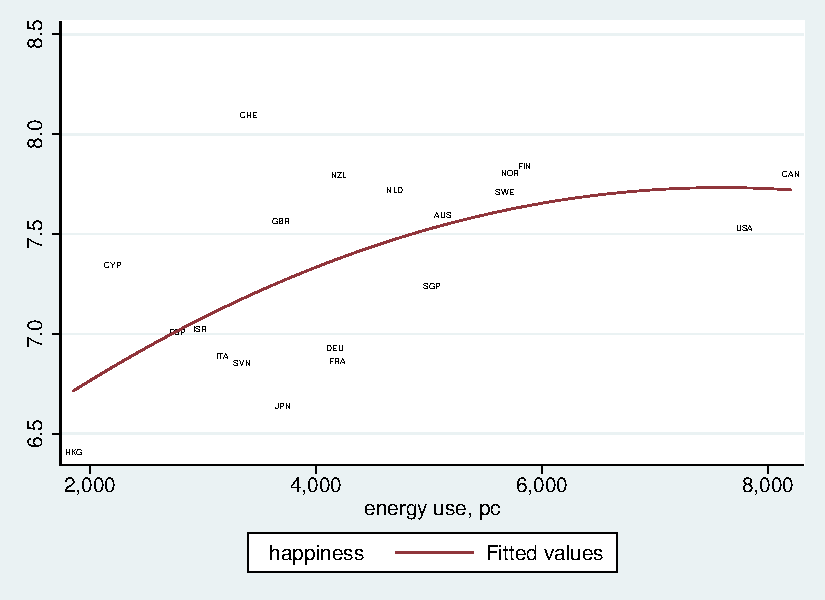
\includegraphics[height=3in]{graphsAndTables/couWvsLsEne.pdf}\centering
\caption{couWvsLsEne.pdf}\label{couWvsLsEne.pdf}
\end{figure}
{\scriptsize Note: Country codes are in table \ref{ls} in supplementary
  material. If country was observed in more than one year, the data were averaged.}

What is striking is the differences in energy use by area. Diferences are
severalfold. Mexico and Columbia
consume only ??? and yet are as happy as ??? which consumes ???.
 
Table \ref{ls} in supplemenary material lists all countries along with
happiness, energy use and other key variables.

It is critical to control for percoent urban or population density, because
urban or dense areas are less happy and more energy efficient, and hence
omission of this variable leads to positive bias on energy use--the estimated
coefficient   is larger than it should be in a bivariate case. Indeed, bivariate
relationship appears positive. 

The bottom line is that there appears to be weak relationship betwen electricity
consumption and happiness, but it disappears or indeed becomes negative when
taking into account social support. One explanation is that people who consumer
more electricity, need to work more, and have less time for social stuff which
is iomportant for happiness. Per Bowling Alone, we do less and less social stuff
and robert frank--need to focus on non-pecuniary domain!

Regression results are set in table \ref{regA}. First we start with an ols
model. All ols regressions control for year dummies--again, different countries
were surveyed in different years. Energy consumption results in greater
happiness (ols1), but when controlling for PCGDP, the relationship disappears
(ols2). Addition of percent urban, unemployment rate and life expectancy (ols3)
makes the relationship actually significantly negative.  Addition of maximum
temperatures in January and July (ols4) makes it positive again but still
insignificant.  A very interesting thing occurs in column ols5--addition of
$CO_2$ makes energy positive and significant.\footnote{The two variables are
  correlated at .91. And $CO_2$ is negative as expected. Energy correlates at .38
  with happiness, and $CO_2$ correlates at .29 (positive, too).}
 Hence, energy consumption would increase happiness if not emissions. This may
 point to clean energy (wind, solar, etc) as a solution. 

Furthemore, in such a diverse sample of countries, there is some unobserved
heterogeneity. Two fixed effects model follow (temperature drops out, because we
 only have temperature for country for one time period). Yet comfortingly
 results are similar to ols, when not controling for $CO_2$, results ar weakly
 positive (fe1), but when adding $CO_2$ control results become significant
 (fe2). Again, we intrpret it  that energy consumption WITHOUT pollution would
 contribute more to happiness than just energy consumption.  

\begin{table}[H]\centering \caption{regA} \label{regA} \begin{scriptsize} \begin{tabular}{p{1.4in}p{.43in}p{.43in}p{.43in}p{.43in}p{.43in}p{.43in}p{.43in}p{.43in}p{.43in}p{.43 in}p{.43in}p{.43 in}}\hline                     &        ols1   &        ols2   &        ols3   &        ols4   &        ols5   &         fe1   &         fe2   \\
energy use, pc      &       0.000***&      -0.000+  &      -0.000*  &       0.000   &       0.000** &       0.001+  &       0.001*  \\
PCGDP               &               &       0.000***&       0.000***&       0.000** &       0.000*  &       0.000   &      -0.000   \\
percent urban       &               &               &       0.018** &      -0.001   &      -0.001   &       0.019   &       0.030   \\
unemployment, \%     &               &               &      -0.026*  &      -0.008   &      -0.002   &       0.010   &       0.009   \\
female life expectancy&               &               &       0.006   &       0.050** &       0.057***&      -0.002   &      -0.003   \\
maximum temperature in January&               &               &               &       0.045***&       0.049***&               &               \\
maximum temperature in July&               &               &               &      -0.019*  &      -0.014   &               &               \\
co2 emissions, pc   &               &               &               &               &      -0.108** &               &      -0.262   \\
constant            &       6.592***&       6.693***&       5.473***&       2.725*  &       1.921   &       3.657   &       3.245   \\
N                   &         163   &         162   &         139   &         139   &         139   &         139   &         139   \\
 \hline\multicolumn{6}{l}{+p$<$0.10 *p$<$0.05 **p$<$0.01 ***p$<$0.001; robust standard errors} \end{tabular}\end{scriptsize}\end{table}
 

\section{Conclusion and Discussion}

Hence, the messgae of this study is that if we change from society of consumers
to socitty of conservers, we won't suffer much in terms of happiness.

Much, and  arguably most among the rich, of the consumption is conspicous or
wasteful \citep{veblen05a, veblen05b}--that is, such consumption is done not to satisfy need but to show that
one is better than others--many of these consumption items waste energy: for
instance: Mansions, SUVs.  Many other examples are not necessarily conspicous
but they waste energy and have no clear contribution to lasting happiness: for
instance landscaping, fake (unnatural) ponds fountains and other items that
define American suburbia. Many social scientists \citep[e.g.][]{csikszentmihalyi99, frank04, frank05, frank12} suggested that conspicuous consumption
does not make us any happier, and there are theoretical reasons to
expect it, but few actually test it--and again, the only  study testing the
effect of energy use on happiness was \citet{graef81}.

One implication of the study is for housing: house is most expensive consumption
item most people buy. Furthermore it costs considerable energy to build and
maintain. The median house in 1973 was 1,525 sq ft, and 2,169  sq ft in 2010.\footnote{\url{http://www.census.gov/const/C25Ann/sftotalmedavgsqft.pdf}}
Surely, the families must have gotten bigger over that time. Well,
actually they gotten smaller--in 1973 the average household size was
3.01, which dropped to 2.61 in
2010.\footnote{\url{http://www.census.gov/population/socdemo/hh-fam/tabHH-6.pdf};\url{http://quickfacts.census.gov/qfd/states/00000.html}}
The problem with big houses is that it is never big enough anyway--we
compare it to other houses, and size is an obvious metric. But others
do the same and they get ever bigger houses all the time so we all end
up with bigger houses but nobody is happier \citep{frank12}. ``A house may be large or small; as long as the neighboring houses are
likewise small, it satisfies all social requirements for a
residence. But let there arise next to the little house a palace, and
the little house shrinks to a hut'' (Marx and Engels 1849, quoted in
\citet{dittmann10}). \citet{dittmann10} find support for the above
statement. \citet{luttmer05} also finds that the richer the neighbors,
the less happy the person.
\citet{firebaugh09} refine this relationship by confirming that people
are happier in poor counties, but in  rich neighborhoods. 

We find that energy consumption does contribute to happiess, if pollution is
taken into account. This is a clear argument in favor of clean energy--if we can
consume energy without pollution, it should result in greater happiness. Untill
we can to do so for all of our energy needs, we should curb the energy use and
our needs.

\section{Future Research}

There are many ideas for future research. Indeed, as mentioned earlier, one of
the goals of this study is to encourage more research on this important and
overlooked topic of energy consumption and happiness.

We just examined total energy use per capita at country level without
differentiating between sectors, because we could not find ssuch data. There are
however enrgy use data by sector for smaller sets of countries--for instance for
Europe available from Eurostat: 
\url{http://epp.eurostat.ec.europa.eu/portal/page/portal/energy/data/database}, \url{http://epp.eurostat.ec.europa.eu/portal/page/portal/energy/data/main_tables} 

We suggest that clean energy would result in greater happiness. This idea could
poissibly be tested more direcly by examining happiness of people in areas where
clean energy is prevalent. 


Yet, energy efficiency or even clean energy is not the final solution due to
``rebound problem'' or the Jevons paradox--due to innate human greed we are
likely to consume ever more and more, and hence the only lasting solution is to
curb our energy hunger possibly through public policy and education.

\newpage
%\bibliography{/home/aok/papers/root/tex/ebib.bib}

\begin{thebibliography}{36}
\newcommand{\enquote}[1]{``#1''}
\expandafter\ifx\csname natexlab\endcsname\relax\def\natexlab#1{#1}\fi

\bibitem[\protect\citeauthoryear{Brickman, Coates, and Janoff-Buman}{Brickman
  et~al.}{1978}]{brickman78cj}
\textsc{Brickman, P., D.~Coates, and R.~Janoff-Buman} (1978): \enquote{Lottery
  winners and accident victims: Is happiness relative?} \emph{Journal of
  Personality and Social Psychology}, 36, 917--927.

\bibitem[\protect\citeauthoryear{Brown and Kasser}{Brown and
  Kasser}{2005}]{brown05}
\textsc{Brown, K.~W. and T.~Kasser} (2005): \enquote{Are psychological and
  ecological well-being compatible? The role of values, mindfulness, and
  lifestyle,} \emph{Social Indicators Research}, 74, 349--368.

\bibitem[\protect\citeauthoryear{Corral-Verdugo, Mireles-Acosta, Tapia-Fonllem,
  and Fraijo-Sing}{Corral-Verdugo et~al.}{2011}]{corral11}
\textsc{Corral-Verdugo, V., J.~Mireles-Acosta, C.~Tapia-Fonllem, and
  B.~Fraijo-Sing} (2011): \enquote{Happiness as correlate of sustainable
  behavior: A study of pro-ecological, frugal, equitable and altruistic actions
  that promote subjective wellbeing,} \emph{Human Ecology Review}, 18, 95--104.

\bibitem[\protect\citeauthoryear{Csikszentmihalyi}{Csikszentmihalyi}{1999}]{csikszentmihalyi99}
\textsc{Csikszentmihalyi, M.} (1999): \enquote{If we are so rich, why aren't we
  happy?} \emph{American psychologist}, 54, 821.

\bibitem[\protect\citeauthoryear{Csikszentmihalyi, Graef, and
  Gianinno}{Csikszentmihalyi et~al.}{2014}]{csikszentmihalyi14}
\textsc{Csikszentmihalyi, M., R.~Graef, and S.~M. Gianinno} (2014):
  \enquote{Energy Consumption in Leisure and Perceived Happiness,} in
  \emph{Flow and the Foundations of Positive Psychology}, Springer, 127--133.

\bibitem[\protect\citeauthoryear{Daly}{Daly}{2013}]{daly13}
\textsc{Daly, H.} (2013): \enquote{A further critique of growth economics,}
  \emph{Ecological economics}, 88, 20--24.

\bibitem[\protect\citeauthoryear{Dias, Mattos, and P~Balestieri}{Dias
  et~al.}{2006}]{dias06}
\textsc{Dias, R.~A., C.~R. Mattos, and J.~A. P~Balestieri} (2006): \enquote{The
  limits of human development and the use of energy and natural resources,}
  \emph{Energy Policy}, 34, 1026--1031.

\bibitem[\protect\citeauthoryear{Diener}{Diener}{2009}]{diener09}
\textsc{Diener, E.} (2009): \emph{Well-being for public policy}, Oxford
  University Press.

\bibitem[\protect\citeauthoryear{Dietz, Rosa, and York}{Dietz
  et~al.}{2009}]{dietz09}
\textsc{Dietz, T., E.~A. Rosa, and R.~York} (2009): \enquote{Environmentally
  efficient well-being: Rethinking sustainability as the relationship between
  human well-being and environmental impacts,} \emph{Human Ecology Review}, 16,
  114--123.

\bibitem[\protect\citeauthoryear{Dittmann and Goebel}{Dittmann and
  Goebel}{2010}]{dittmann10}
\textsc{Dittmann, J. and J.~Goebel} (2010): \enquote{{Your House, Your Car,
  Your Education: The Socioeconomic Situation of the Neighborhood and its
  Impact on Life Satisfaction in Germany},} \emph{Social Indicators Research},
  1--17.

\bibitem[\protect\citeauthoryear{Durkheim}{Durkheim}{[1895] 1950}]{durkheim50}
\textsc{Durkheim, E.} ([1895] 1950): \emph{The Rules of Sociological Method},
  New York: The Free Press.

\bibitem[\protect\citeauthoryear{Ericson, Kj{\o}nstad, and Barstad}{Ericson
  et~al.}{2014}]{ericson14}
\textsc{Ericson, T., B.~G. Kj{\o}nstad, and A.~Barstad} (2014):
  \enquote{Mindfulness and sustainability,} \emph{Ecological Economics}, 104,
  73--79.

\bibitem[\protect\citeauthoryear{Firebaugh and Schroeder}{Firebaugh and
  Schroeder}{2009}]{firebaugh09}
\textsc{Firebaugh, G. and M.~B. Schroeder} (2009): \enquote{Does Your
  Neighbor's Income Affect Your Happiness?} \emph{American Journal of
  Sociology}, 115, 805--831.

\bibitem[\protect\citeauthoryear{Frank}{Frank}{2012}]{frank12}
\textsc{Frank, R.} (2012): \emph{The Darwin economy: Liberty, competition, and
  the common good}, Princeton University Press.

\bibitem[\protect\citeauthoryear{Frank}{Frank}{2004}]{frank04}
\textsc{Frank, R.~H.} (2004): \enquote{How not to buy happiness,}
  \emph{Daedalus}, 133, 69--79.

\bibitem[\protect\citeauthoryear{Frank}{Frank}{2005}]{frank05}
---\hspace{-.1pt}---\hspace{-.1pt}--- (2005): \enquote{Does Absolute Income
  Matter,} in \emph{Economics and Happiness}, ed. by L.~Bruni and P.~L. Porta,
  Oxford University Press.

\bibitem[\protect\citeauthoryear{Graef, McManama~Gianinno, and
  Csikszentmihalyi}{Graef et~al.}{1981}]{graef81}
\textsc{Graef, R., S.~McManama~Gianinno, and M.~Csikszentmihalyi} (1981):
  \enquote{Energy consumption in leisure and perceived happiness,} in
  \emph{Consumers and energy conservation}, ed. by J.~M. Claxton, New York:
  Praeger, --.

\bibitem[\protect\citeauthoryear{Jorgenson, Alekseyko, and
  Giedraitis}{Jorgenson et~al.}{2014}]{jorgenson14B}
\textsc{Jorgenson, A.~K., A.~Alekseyko, and V.~Giedraitis} (2014):
  \enquote{Energy consumption, human well-being and economic development in
  central and eastern European nations: A cautionary tale of sustainability,}
  \emph{Energy Policy}, 66, 419--427.

\bibitem[\protect\citeauthoryear{Kallis}{Kallis}{2011}]{kallis11}
\textsc{Kallis, G.} (2011): \enquote{In defence of degrowth,} \emph{Ecological
  Economics}, 70, 873--880.

\bibitem[\protect\citeauthoryear{Kallis, Kerschner, and Martinez-Alier}{Kallis
  et~al.}{2012}]{kallis12}
\textsc{Kallis, G., C.~Kerschner, and J.~Martinez-Alier} (2012): \enquote{The
  economics of degrowth,} \emph{Ecological Economics}, 84, 172--180.

\bibitem[\protect\citeauthoryear{Klugman, Rodr{\'\i}guez, and Choi}{Klugman
  et~al.}{2011}]{klugman11}
\textsc{Klugman, J., F.~Rodr{\'\i}guez, and H.-J. Choi} (2011): \enquote{The
  HDI 2010: new controversies, old critiques,} \emph{The Journal of Economic
  Inequality}, 9, 249--288.

\bibitem[\protect\citeauthoryear{Luttmer}{Luttmer}{2005}]{luttmer05}
\textsc{Luttmer, E. F.~P.} (2005): \enquote{Neighbors as Negatives: Relative
  Earnings and Well-Being,} \emph{Quarterly Journal of Economics}, 120,
  963--02.

\bibitem[\protect\citeauthoryear{Madjar and Ozawa}{Madjar and
  Ozawa}{2006}]{madjar06}
\textsc{Madjar, M. and T.~Ozawa} (2006): \enquote{Happiness and Sustainable
  Consumption: Psychological and physical rebound effects at work in a tool for
  sustainable design,} \emph{The International Journal of Life Cycle
  Assessment}, 11, 105--115.

\bibitem[\protect\citeauthoryear{Michalos}{Michalos}{1985}]{michalos85}
\textsc{Michalos, A.} (1985): \enquote{Multiple discrepancies theory (MDT),}
  \emph{Social Indicators Research}, 16, 347--413.

\bibitem[\protect\citeauthoryear{Pretty}{Pretty}{2013}]{pretty13}
\textsc{Pretty, J.} (2013): \enquote{The consumption of a finite planet:
  well-being, convergence, divergence and the nascent green economy,}
  \emph{Environmental and Resource Economics}, 55, 475--499.

\bibitem[\protect\citeauthoryear{Steel, Schmidt, and Shultz}{Steel
  et~al.}{2008}]{steel08}
\textsc{Steel, P., J.~Schmidt, and J.~Shultz} (2008): \enquote{Refining the
  relationship between personality and subjective well-being.}
  \emph{Psychological bulletin}, 134, 138--161.

\bibitem[\protect\citeauthoryear{Steinberger and Roberts}{Steinberger and
  Roberts}{2010}]{steinberger10}
\textsc{Steinberger, J.~K. and J.~T. Roberts} (2010): \enquote{From constraint
  to sufficiency: The decoupling of energy and carbon from human needs,
  1975--2005,} \emph{Ecological Economics}, 70, 425--433.

\bibitem[\protect\citeauthoryear{Stiglitz, Sen, and Fitoussi}{Stiglitz
  et~al.}{2009}]{stiglitz09al}
\textsc{Stiglitz, J., A.~Sen, and J.~Fitoussi} (2009): \enquote{Report by the
  Commission on the measurement of economic performance and social progress,}
  \emph{Available at www.stiglitz-sen-fitoussi.fr}.

\bibitem[\protect\citeauthoryear{Van~den Bergh}{Van~den Bergh}{2011}]{bergh11}
\textsc{Van~den Bergh, J.~C.} (2011): \enquote{Environment versus growth--A
  Criticism of "degrowth" and a plea for "a-growth",} \emph{Ecological
  Economics}, 70, 881--890.

\bibitem[\protect\citeauthoryear{Veenhoven}{Veenhoven}{1996}]{veenhoven96B}
\textsc{Veenhoven, R.} (1996): \enquote{Happy life-expectancy,} \emph{Social
  Indicators Research}, 39, 1--58.

\bibitem[\protect\citeauthoryear{Veenhoven}{Veenhoven}{2008}]{veenhoven08}
---\hspace{-.1pt}---\hspace{-.1pt}--- (2008): \enquote{Sociological theories of
  subjective well-being,} in \emph{The Science of Subjective Well-being: A
  tribute to Ed Diener}, ed. by M.~Eid and R.~Larsen, The Guilford Press, New
  York, 44--61.

\bibitem[\protect\citeauthoryear{Veenhoven}{Veenhoven}{2014}]{veenhoven14b}
---\hspace{-.1pt}---\hspace{-.1pt}--- (2014): \enquote{Livability Theory,}
  \emph{Encyclopedia of Quality of Life and Well-Being Research}, 3645--3647.

\bibitem[\protect\citeauthoryear{Veenhoven and Ehrhardt}{Veenhoven and
  Ehrhardt}{1995}]{veenhoven95}
\textsc{Veenhoven, R. and J.~Ehrhardt} (1995): \enquote{The Cross-National
  Pattern of Happiness: Test of Predictions Implied in Three Theories of
  Happiness,} \emph{Social Indicators Research}, 34, 33--68.

\bibitem[\protect\citeauthoryear{Weinhold}{Weinhold}{2012}]{weinhold12}
\textsc{Weinhold, D.} (2012): \enquote{The Happiness-Reducing Costs of Noise
  Pollution,} \emph{Journal of regional science}.

\bibitem[\protect\citeauthoryear{Welsch}{Welsch}{2005}]{welsch05}
\textsc{Welsch, H.} (2005): \enquote{Environment and happiness: Valuation of
  air pollution using life satisfaction data,} \emph{Ecological Economics}, 58,
  801--813.

\bibitem[\protect\citeauthoryear{Welsch}{Welsch}{2009}]{welsch09}
---\hspace{-.1pt}---\hspace{-.1pt}--- (2009): \enquote{Implications of
  happiness research for environmental economics,} \emph{Ecological Economics},
  68, 2735--2742.

\end{thebibliography}



\newpage
\section{ONLINE SUPPLEMENATRY MATERIAL}

 \begin{scriptsize}  \begin{center} \begin{longtable}{llllllllllllll} \caption{
Key
variables
for
each
country.}
\label{ls}
\\
\hline
\multicolumn{1}{p{.75in}}{Country
Code
(ISO
2
digits)}
&
\multicolumn{1}{p{.75in}}{Country
Name}
&
\multicolumn{1}{p{.75in}}{happiness
(WDH)}&
\multicolumn{1}{p{.75in}}{energy
use,
pc}&
\multicolumn{1}{p{.75in}}{PCGDP}&
\multicolumn{1}{p{.75in}}{co2
emissions,
pc}&
\multicolumn{1}{p{.75in}}{female
life
expectancy}
&
\multicolumn{1}{p{.75in}}{}
\\
\hline
\endfirsthead
\multicolumn{3}{p{.75in}}
{{\bfseries
\tablename\
\thetable{}
--
continued
from
previous
page}}
\\
\hline
\multicolumn{1}{p{.75in}}{Country
Code
(ISO
2
digits)}
&
\multicolumn{1}{p{.75in}}{Country
Name}
&
\multicolumn{1}{p{.75in}}{happiness
(WDH)}&
\multicolumn{1}{p{.75in}}{energy
use,
pc}&
\multicolumn{1}{p{.75in}}{PCGDP}
&
\multicolumn{1}{p{.75in}}{co2
emissions,
pc}&
\multicolumn{1}{p{.75in}}{female
life
expectancy}
&
\multicolumn{1}{p{.75in}}{}\\
\hline
\endhead
\hline
\multicolumn{5}{r}{{Continued
on
next
page}}
\\
\endfoot
\hline
\endlastfoot

AD&Andorra&6.8&&31,107&7.1&\\
AE&United Arab Emirates&7.3&10,447&40,623&28.0&76\\
AF&Afghanistan&4.1&&267&0.1&58\\
AL&Albania&4.6&671&2,773&1.3&79\\
AM&Armenia&5.0&780&1,551&1.4&76\\
AO&Angola&4.3&589&1,798&1.1&49\\
AR&Argentina&7.3&1,733&5,349&4.1&78\\
AT&Austria&7.4&3,911&37,097&8.4&82\\
AU&Australia&7.7&5,605&33,593&17.6&83\\
AZ&Azerbaijan&5.3&1,467&1,740&4.2&72\\
BA&Bosnia and Herzegovina&5.8&1,289&2,791&6.6&78\\
BD&Bangladesh&5.3&166&421&0.3&68\\
BE&Belgium&7.3&5,544&35,692&10.4&82\\
BF&Burkina Faso&4.4&&395&0.1&53\\
BG&Bulgaria&4.4&2,490&3,651&6.1&76\\
BI&Burundi&2.9&&148&0.0&51\\
BJ&Benin&3.0&327&536&0.4&58\\
BO&Bolivia&6.3&499&1,029&1.3&67\\
BR&Brazil&7.5&1,160&4,771&1.9&75\\
BW&Botswana&4.7&1,046&5,347&2.4&48\\
BY&Belarus&5.2&2,740&3,077&5.9&75\\
BZ&Belize&6.6&604&3,977&1.7&75\\
CA&Canada&7.8&8,106&35,353&16.9&83\\
CD&Congo, Dem. Rep.&4.4&368&220&0.0&49\\
CF&Central African Republic&4.6&&360&0.1&47\\
CG&Congo, Rep.&3.7&302&1,685&0.3&55\\
CH&Switzerland&8.0&3,528&52,041&5.5&84\\
CI&Cote d'Ivoire&4.4&490&956&0.4&48\\
CL&Chile&6.7&1,703&7,452&3.8&81\\
CM&Cameroon&3.9&371&909&0.2&53\\
CN&China&6.3&1,292&1,752&4.1&75\\
CO&Colombia&7.7&634&3,410&1.4&76\\
CR&Costa Rica&8.5&877&4,651&1.6&81\\
CY&Cyprus&7.1&2,249&22,498&7.4&81\\
CZ&Czech Republic&6.5&4,279&12,458&11.8&79\\
DE&Germany&7.1&4,075&34,054&9.8&82\\
DJ&Djibouti&5.7&178&924&0.6&60\\
DK&Denmark&8.3&3,558&46,939&9.1&80\\
DO&Dominican Republic&7.5&771&3,754&2.2&75\\
DZ&Algeria&5.4&961&2,884&3.0&71\\
EC&Ecuador&6.4&742&2,932&2.0&77\\
EE&Estonia&6.0&3,737&9,666&12.1&78\\
EG&Egypt, Arab Rep.&5.7&808&1,278&2.3&72\\
ES&Spain&7.2&3,100&25,523&7.5&84\\
ET&Ethiopia&4.2&382&163&0.1&57\\
FI&Finland&7.9&6,691&36,747&11.4&82\\
FR&France&6.6&4,181&33,576&6.0&84\\
GB&United Kingdom&7.2&3,591&37,282&8.8&81\\
GE&Georgia&4.3&658&1,432&1.1&76\\
GH&Ghana&5.2&403&503&0.4&59\\
GN&Guinea&4.5&&303&0.1&53\\
GR&Greece&6.4&2,645&21,170&8.7&82\\
GT&Guatemala&7.2&625&2,176&0.9&73\\
GY&Guyana&6.5&646&1,097&2.0&68\\
HK&Hong Kong SAR, China&6.6&2,003&25,951&5.7&85\\
HN&Honduras&7.0&566&1,383&1.0&74\\
HR&Croatia&6.0&1,952&9,815&5.1&79\\
HT&Haiti&3.9&264&466&0.2&61\\
HU&Hungary&5.5&2,587&10,409&5.6&77\\
ID&Indonesia&6.3&785&1,268&1.5&71\\
IE&Ireland&7.6&3,484&46,692&10.4&81\\
IL&Israel&7.0&2,894&19,659&9.5&82\\
IN&India&5.5&486&735&1.3&65\\
IQ&Iraq&4.7&999&1,874&3.4&73\\
IR&Iran, Islamic Rep.&5.9&2,359&2,690&6.7&73\\
IS&Iceland&8.2&13,136&52,394&7.3&83\\
IT&Italy&6.7&3,049&30,633&7.9&84\\
JM&Jamaica&6.7&1,439&4,190&4.1&74\\
JO&Jordan&5.9&1,140&2,315&3.5&74\\
JP&Japan&6.5&3,992&35,282&9.5&86\\
KE&Kenya&3.7&451&525&0.3&56\\
KG&Kyrgyz Republic&5.5&487&484&1.0&72\\
KH&Cambodia&4.9&281&457&0.2&69\\
KR&Korea, Rep.&6.0&4,343&18,350&9.9&82\\
KW&Kuwait&6.6&10,513&32,141&29.0&75\\
KZ&Kazakhstan&6.1&3,371&3,595&11.7&72\\
LA&Lao PDR&6.2&&471&0.2&65\\
LB&Lebanon&4.7&1,366&5,590&4.4&79\\
LK&Sri Lanka&5.1&447&1,245&0.6&77\\
LR&Liberia&4.3&&191&0.2&56\\
LT&Lithuania&5.5&2,649&7,487&4.1&78\\
LU&Luxembourg&7.7&8,552&79,226&22.1&82\\
LV&Latvia&5.4&1,947&6,746&3.2&77\\
MA&Morocco&5.4&422&1,947&1.4&71\\
MD&Moldova&4.9&905&786&1.2&72\\
ME&Montenegro&5.2&1,736&3,781&3.6&77\\
MG&Madagascar&3.7&&280&0.1&62\\
MK&Macedonia, FYR&4.7&1,340&2,890&5.5&76\\
ML&Mali&4.7&&443&0.0&51\\
MN&Mongolia&5.7&1,092&987&3.5&69\\
MR&Mauritania&4.9&&705&0.5&62\\
MT&Malta&7.1&2,010&15,024&6.2&82\\
MW&Malawi&6.2&&219&0.1&49\\
MX&Mexico&7.9&1,480&7,809&3.8&78\\
MY&Malaysia&6.5&2,334&5,457&6.6&76\\
MZ&Mozambique&3.8&404&303&0.1&49\\
NA&Namibia&5.2&604&3,506&1.1&59\\
NE&Niger&3.8&&263&0.1&54\\
NG&Nigeria&5.7&742&749&0.7&49\\
NI&Nicaragua&7.1&509&1,147&0.8&75\\
NL&Netherlands&7.6&4,760&39,400&10.5&82\\
NO&Norway&7.9&5,880&64,397&9.3&82\\
NP&Nepal&5.3&358&322&0.1&65\\
NZ&New Zealand&7.5&4,191&26,786&8.2&82\\
PA&Panama&7.8&859&4,727&2.0&79\\
PE&Peru&6.2&485&2,713&1.3&75\\
PH&Philippines&5.9&459&1,190&0.9&71\\
PK&Pakistan&5.0&472&672&0.8&66\\
PL&Poland&6.4&2,432&8,036&8.0&79\\
PS&West Bank and Gaza&4.9&&1,247&0.5&73\\
PT&Portugal&5.7&2,400&18,307&5.9&81\\
PY&Paraguay&6.8&696&1,504&0.7&73\\
QA&Qatar&6.8&19,868&54,880&54.2&78\\
RO&Romania&5.7&1,791&4,607&4.4&76\\
RS&Serbia&5.4&2,166&3,261&6.9&76\\
RU&Russian Federation&5.5&4,516&5,210&11.2&73\\
RW&Rwanda&4.3&&271&0.1&56\\
SA&Saudi Arabia&6.5&5,692&13,381&15.5&76\\
SD&Sudan&5.0&384&675&0.3&62\\
SE&Sweden&7.8&5,532&40,050&5.6&83\\
SG&Singapore&6.9&5,454&28,541&7.7&82\\
SI&Slovenia&6.9&3,529&17,647&7.8&81\\
SK&Slovak Republic&5.9&3,393&11,443&7.1&78\\
SL&Sierra Leone&3.5&&315&0.1&42\\
SN&Senegal&4.5&249&752&0.5&62\\
SV&El Salvador&6.7&718&2,790&1.1&75\\
SY&Syrian Arab Republic&5.9&1,046&1,518&2.9&76\\
TD&Chad&5.4&&547&0.0&49\\
TG&Togo&2.6&427&389&0.2&55\\
TH&Thailand&6.6&1,437&2,621&3.7&76\\
TJ&Tajikistan&5.1&341&326&0.4&69\\
TM&Turkmenistan&7.2&3,911&1,769&9.5&69\\
TN&Tunisia&5.9&840&3,214&2.3&76\\
TR&Turkey&5.6&1,265&6,803&3.6&76\\
TT&Trinidad and Tobago&7.0&12,286&12,048&25.7&73\\
TZ&Tanzania&2.8&429&367&0.1&54\\
UA&Ukraine&5.0&2,866&1,734&6.8&74\\
UG&Uganda&4.8&&319&0.1&53\\
US&United States&7.4&7,725&43,146&19.3&80\\
UY&Uruguay&6.7&940&5,310&1.8&79\\
UZ&Uzbekistan&6.0&1,910&552&4.6&71\\
VE&Venezuela, RB&7.5&2,313&5,503&6.7&76\\
VN&Vietnam&6.1&485&685&1.1&79\\
YE&Yemen, Rep.&4.8&313&820&1.0&63\\
ZA&South Africa&5.8&2,658&5,149&8.7&55\\
ZM&Zambia&5.0&621&626&0.2&47\\
ZW&Zimbabwe&3.0&743&498&0.8&45\\
\end{longtable} \end{center} \end{scriptsize}   


\end{spacing}
\end{document}
